\documentclass[11pt]{article}

\usepackage[T1]{fontenc}
\usepackage{lmodern}
\usepackage[margin=2cm]{geometry}
\usepackage{amsmath,amssymb}
\usepackage{graphicx}
\usepackage{xcolor}
\usepackage{enumitem}
\usepackage{fancyhdr}
\usepackage{pgfplots}
\pgfplotsset{compat=1.17}

% Colors
\definecolor{titleblue}{RGB}{31,56,100}
\definecolor{headergray}{RGB}{110,110,110}
\definecolor{plotred}{RGB}{176,60,60}

% Header and footer
\pagestyle{fancy}
\fancyhf{}
\fancyhead[L]{\small\color{headergray}MATH 407 \textbar{} Homework 1}
\fancyhead[R]{\small\color{headergray}Yazan Ismail}
\fancyfoot[C]{\thepage}
\renewcommand{\headrulewidth}{0.4pt}

% Paragraph spacing
\setlength{\parindent}{0pt}
\setlength{\parskip}{4pt}

\begin{document}

\begin{center}
  {\Large\bfseries\color{titleblue} Homework 1 - Solutions}\\[2pt]
  Problems 1, 2, and 3
\end{center}

%==================================================
\section*{Problem 1}

\textbf{(a) Feasible region.}
In the first quadrant, the feasible points lie below the lines $5x + 2y = 10$ and $3x + 4y = 12$, and above the line $y = x - 1$. The boundary segments in the Desmos graph enclose a feasible polygon with vertices in boundary order
\[
(0,0), \quad (1,0), \quad \left(\frac{12}{7}, \frac{5}{7}\right), \quad \left(\frac{8}{7}, \frac{15}{7}\right), \quad (0,3).
\]

\begin{center}
  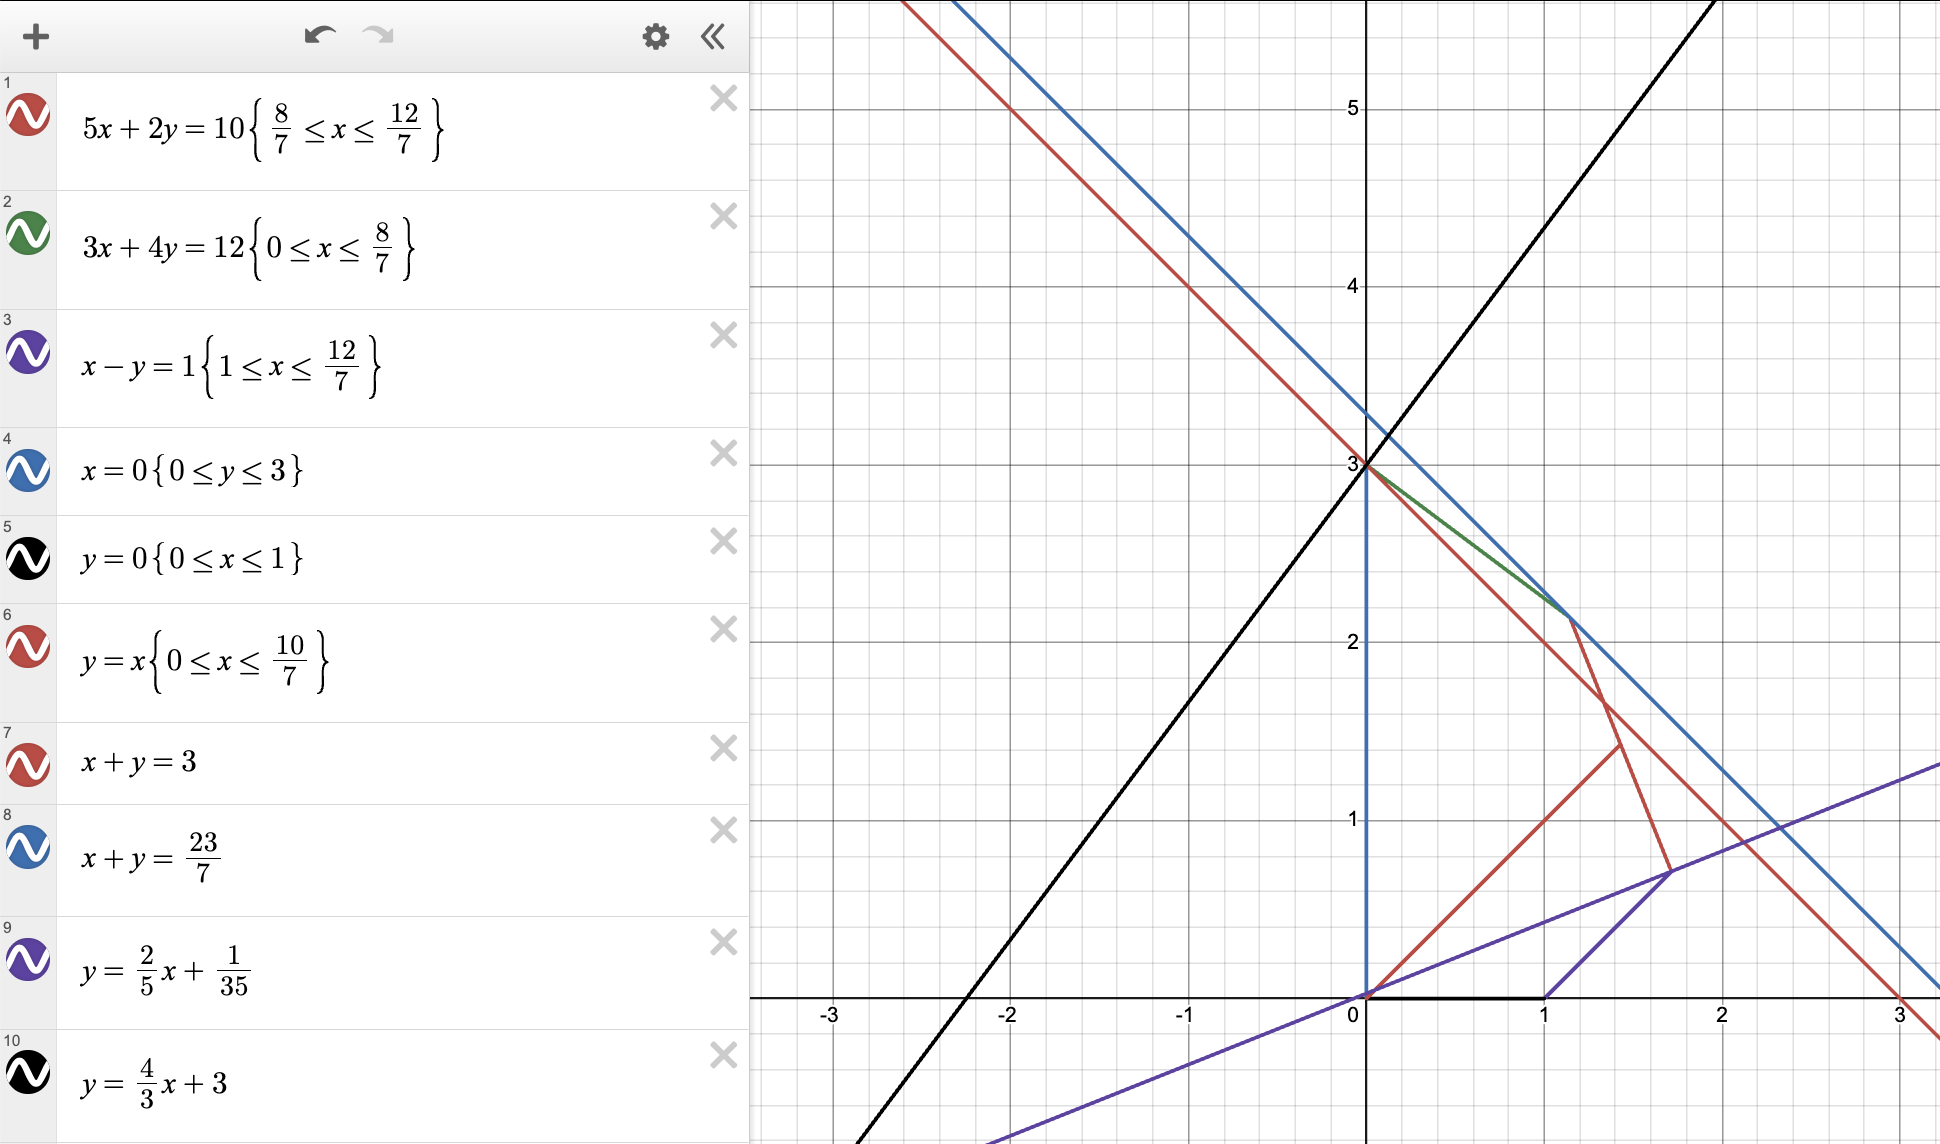
\includegraphics[width=0.5\textwidth]{MATH_407_HW_1_PROBLEM_1.png}
\end{center}

\textbf{(b) Optimal solution and value.}
The objective lines $x + y = k$ move northeast as $k$ increases. Their last contact with the feasible polygon is the intersection of $5x + 2y = 10$ and $3x + 4y = 12$. Solving these equations gives $7x = 8$, hence
\[
(x^*, y^*) = \left(\frac{8}{7}, \frac{15}{7}\right), \qquad
\max(x + y) = \frac{8}{7} + \frac{15}{7} = \boxed{\frac{23}{7}}.
\]
This point also satisfies $x - y = -1 \le 1$ and $x, y \ge 0$, so it is feasible.

\textbf{(c) Parameterized objective.}
The two edge directions from $(x^*, y^*)$ are proportional to $(2, -5)$ and $(-4, 3)$. For $(x^*, y^*)$ to remain optimal for $x + \lambda y$, neither edge direction may increase the objective:
\[
(1, \lambda) \cdot (2, -5) = 2 - 5\lambda \le 0, \qquad
(1, \lambda) \cdot (-4, 3) = -4 + 3\lambda \le 0.
\]
Therefore
\[
\boxed{\frac{2}{5} \le \lambda \le \frac{4}{3}}.
\]
Because the feasible polygon is convex, checking the two adjacent edge directions is sufficient. At either endpoint of this interval, the adjacent edge also consists of optimal solutions.

%==================================================
\newpage
\section*{Problem 2}

\textbf{(a) Standard form.}
The equivalent maximization problem is
\[
\begin{array}{rl}
  \text{maximize}   & y - x \\[2pt]
  \text{subject to} & x + 2y \le 10, \\[2pt]
                    & -x - 2y \le -10, \\[2pt]
                    & x \ge 0, \quad y \ge 0.
\end{array}
\]
The first two inequalities together are equivalent to $x + 2y = 10$.

\textbf{(b) Feasible region.}
The equation $x + 2y = 10$ has intercepts $(10, 0)$ and $(0, 5)$. Imposing $x, y \ge 0$ leaves exactly the closed segment joining these two points:
\[
\left\{ (x, y) : y = \frac{10 - x}{2},\ 0 \le x \le 10 \right\}.
\]

\begin{center}
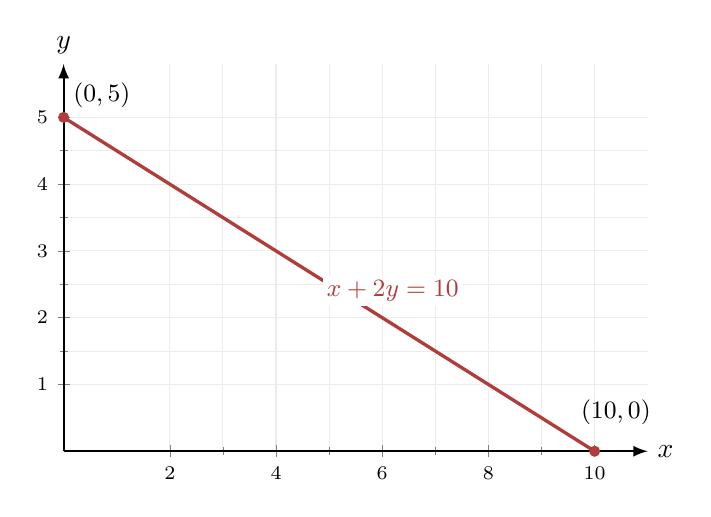
\begin{tikzpicture}
  \begin{axis}[
      width=9cm, height=6.5cm,
      axis lines=middle,
      axis line style={-latex, thick},
      xmin=0, xmax=11, ymin=0, ymax=5.8,
      xtick={2,4,6,8,10}, ytick={1,2,3,4,5},
      minor tick num=1,
      grid=both,
      grid style={gray!15},
      tick label style={font=\scriptsize},
      xlabel={$x$}, ylabel={$y$},
      every axis x label/.style={at={(ticklabel* cs:1)}, anchor=west},
      every axis y label/.style={at={(ticklabel* cs:1)}, anchor=south},
      clip=false
    ]
    \addplot[plotred, very thick, domain=0:10, samples=2] {(10 - x)/2};
    \fill[plotred] (axis cs:0,5) circle (2pt);
    \fill[plotred] (axis cs:10,0) circle (2pt);
    \node[anchor=south west, font=\small] at (axis cs:0,5) {$(0,5)$};
    \node[anchor=south, font=\small] at (axis cs:10.4,0.25) {$(10,0)$};
    \node[plotred, fill=white, inner sep=1.5pt, font=\small] at (axis cs:6.2,2.4) {$x + 2y = 10$};
  \end{axis}
\end{tikzpicture}
\end{center}

\textbf{(c) Optimal solution and value.}
On the segment, $y = (10 - x)/2$, so
\[
x - y = x - \frac{10 - x}{2} = \frac{3x - 10}{2}.
\]
This expression increases with $x$ on $0 \le x \le 10$. Thus its minimum occurs at $x = 0$, giving
\[
\boxed{(x^*, y^*) = (0, 5)}, \qquad \boxed{\min(x - y) = -5}.
\]

\textbf{(d) Independent modifications.}
Each item below changes the original problem separately.
\begin{enumerate}[label=(\roman*), leftmargin=*, itemsep=2pt]
  \item Add $x + 2y = 5$. This contradicts the existing equality $x + 2y = 10$, so the LP is infeasible.
  \item Remove $x \ge 0$. Setting $y = t \ge 0$ and $x = 10 - 2t$ gives feasible points with objective $x - y = 10 - 3t \to -\infty$ as $t \to \infty$. Hence the minimization LP is unbounded below.
  \item Add $y = 2x$. Combining it with $x + 2y = 10$ yields $5x = 10$, so $(2, 4)$ is the only feasible point.
  \item Replace the objective by $\max(x + 2y)$. Every point on the feasible segment satisfies $x + 2y = 10$. Therefore all points on that segment are optimal, with optimal value $10$.
\end{enumerate}

%==================================================
\newpage
\section*{Problem 3}

\textbf{(a) Linear optimization model.}
Let $a, b, c, d, e$ denote kilograms of apples, bananas, carrots, dates, and powdered egg whites, respectively. Set
\[
x = \begin{pmatrix} a \\ b \\ c \\ d \\ e \end{pmatrix}, \qquad
A = \begin{pmatrix}
  0  & 0   & 8   & 0   & 0    \\
  46 & 123 & 60  & 4   & 0    \\
  60 & 50  & 330 & 390 & 1040 \\
  24 & 46  & 28  & 80  & 0    \\
  3  & 7   & 9   & 25  & 800
\end{pmatrix}, \qquad
n = \begin{pmatrix} 1 \\ 30 \\ 400 \\ 15 \\ 15 \end{pmatrix}, \qquad
p = \begin{pmatrix} 4 \\ 2 \\ 3 \\ 10 \\ 70 \end{pmatrix}.
\]
The entries of $Ax$ are the totals of vitamin A, vitamin C, calcium, fiber, and protein, in that order. The first three totals and requirements are measured in mg; the last two are measured in g. The price vector $p$ is measured in dollars per kg. The required LP is
\[
\boxed{
\begin{array}{rl}
  \text{minimize}   & p^T x = 4a + 2b + 3c + 10d + 70e \\[2pt]
  \text{subject to} & Ax \ge n, \\[2pt]
                    & x \ge 0.
\end{array}
}
\]
The inequality $Ax \ge n$ is componentwise, giving the five explicit requirements
\begin{align*}
  8c &\ge 1, \\
  46a + 123b + 60c + 4d &\ge 30, \\
  60a + 50b + 330c + 390d + 1040e &\ge 400, \\
  24a + 46b + 28c + 80d &\ge 15, \\
  3a + 7b + 9c + 25d + 800e &\ge 15.
\end{align*}

\textbf{(b) Feasibility.}
The carrot column of $A$ has a positive coefficient in every nutrient row. Because there is no upper bound on the amount of carrots, choosing only carrots with amount
\[
c \ge \max\left\{ \frac{1}{8}, \frac{30}{60}, \frac{400}{330}, \frac{15}{28}, \frac{15}{9} \right\} = \frac{5}{3}
\]
meets all five requirements. In particular, for $x = (0, 0, 5/3, 0, 0)^T \ge 0$,
\[
Ax = \begin{pmatrix} 40/3 \\ 100 \\ 550 \\ 140/3 \\ 15 \end{pmatrix}
\ge \begin{pmatrix} 1 \\ 30 \\ 400 \\ 15 \\ 15 \end{pmatrix} = n.
\]
Therefore the feasible set is nonempty, and the LP is feasible.

\vspace{1.5em}
\textbf{(c)}

\vspace{6em}
\textbf{(d)}

\end{document}
